\documentclass[xetex,mathserif,serif]{beamer}

\usepackage{beamerthemesplit}
\usepackage{amsmath}
\usepackage{lmodern}
\usetheme{Rochester}
\usecolortheme{lily}

\usepackage{minted}
\setminted{autogobble, mathescape}
\usemintedstyle{tango}

\title{Pragmatic \LaTeX}
\author{Nicholas Lantz}
\institute{CSM Linux User's Group}
\date{October 20, 2016}

\begin{document}
\maketitle

\begin{frame}
    \frametitle{What is \LaTeX?}

    \begin{itemize}
        \item
            A typesetting and document preparation system
        \item
            Looks better than Word
        \item
            Written especially for writing technical reports
    \end{itemize}
\end{frame}

\begin{frame}
    \frametitle{Ligatures}
    \framesubtitle{\LaTeX{} Vs. Word}

    \begin{itemize}
        \item
            Certain character combinations look awkward together, for
            example\ldots
    \end{itemize}

    \Large
    find vs. {f}ind\\
    fly vs. {f}ly\\
    efficient vs. e{f}{f}{i}ccient
\end{frame}

\begin{frame}
    \frametitle{Typesetting Math}
    \framesubtitle{\LaTeX{} Vs. Word}

    \begin{itemize}
        \item
            We go to Mines, we all need to typeset mathematical equations for
            projects, lab reports, etc.
        \item
            \LaTeX supports these very nicely, and the output looks much better
            than the Word equivalent.
        \item
            We will discuss how to typeset mathematics later.
    \end{itemize}

    \centering
    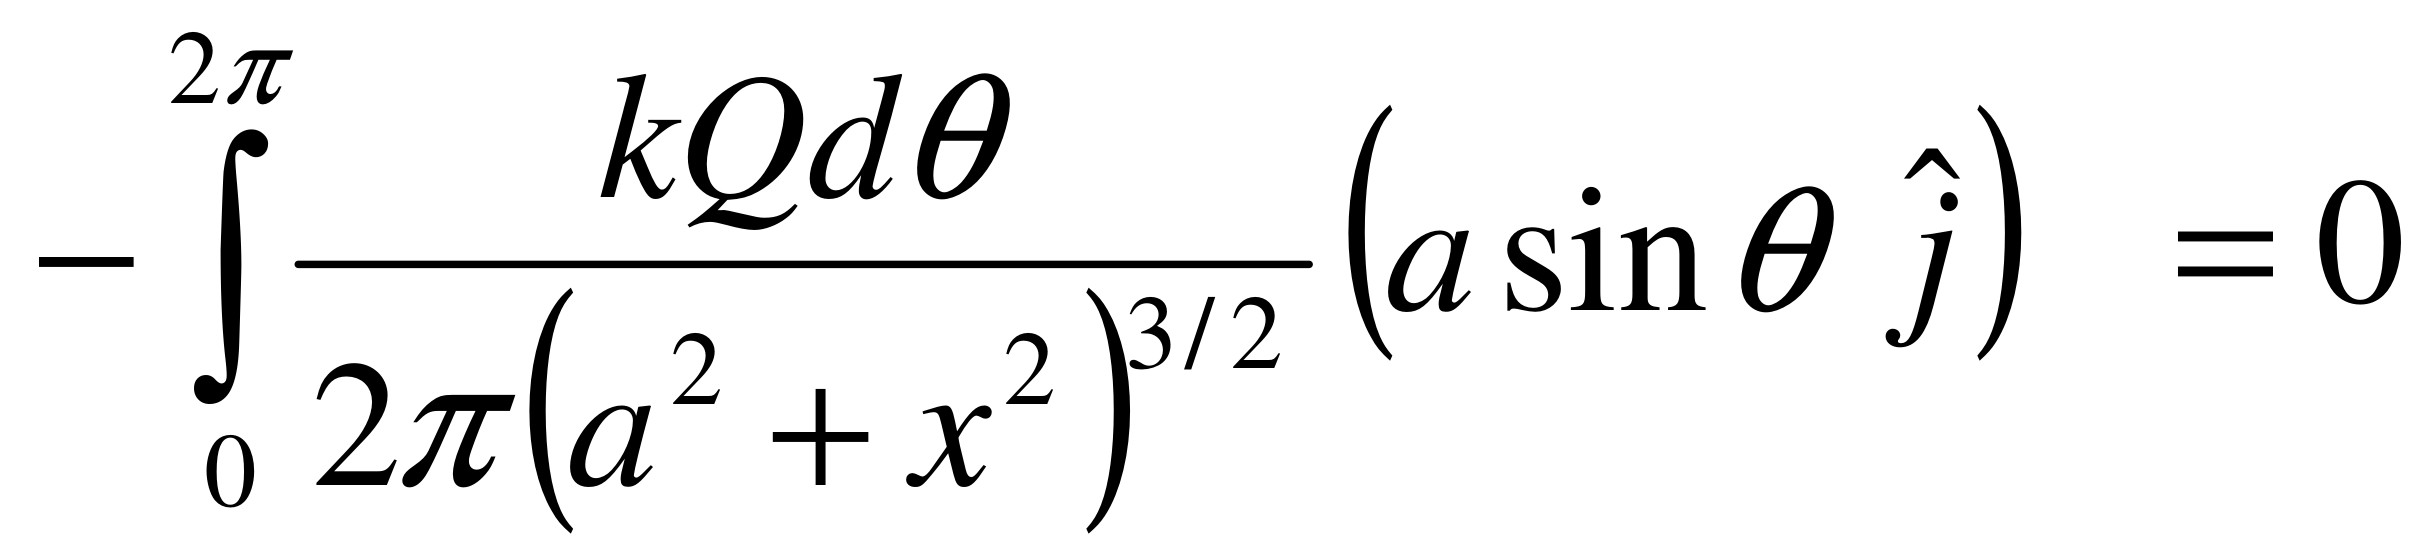
\includegraphics[width=2.5in]{media/wordmath}

    \begin{displaymath}
        -\int_0^{2 \pi} \frac{kQ\, d\theta}{2\pi{\left(a^2 +
        x^2\right)}^{3/2}} (a \sin \theta \,\hat\jmath) = 0
    \end{displaymath}
\end{frame}

\begin{frame}[fragile]
    \frametitle{Structure of \LaTeX{} Document}

    \begin{minted}{Latex}
        \documentclass[letterpaper]{article}

        % Package includes here
        \usepackage[margin=1in]{geometry}

        % Header info here
        \title{Example}
        \author{Nicholas Lantz}
        \date{\today} % Outputs today's date

        \begin{document}
        \maketitle % Creates title based on header info
        % Document goes here....
        \end{document}
    \end{minted}
\end{frame}

\begin{frame}
    \frametitle{Paragraphs}
    \framesubtitle{Writing \LaTeX}

    \begin{itemize}
        \item
            \LaTeX{} considers all spaces between words equally, so adding
            extra spaces between words will not increase the spacing in the
            document.
        \item
            Two ways to create a new paragraph in \LaTeX{}
            \begin{enumerate}
                \item
                    Two newlines (\textbackslash{}n)
                \item
                    \textbackslash{}\textbackslash{}
            \end{enumerate}
        \item
            Generally, use the two newlines, looks better.

        \item
            However, the two wacks can look better inside of the author
            declaration at the top of the document, or in tables (discussed
            later).
    \end{itemize}
\end{frame}

\begin{frame}[fragile]
    \frametitle{Sections}
    \framesubtitle{Writing \LaTeX}

    \begin{minted}{Latex}
        \section{Top-level Section}
        \subsection{Sub-section}
        \section{Yet Another Section}
    \end{minted}

    There are other kinds of sections, like
    \begin{itemize}
        \item
            part
        \item
            chapter
        \item
            section
        \item
            subsection
        \item
            subsubsection
        \item
            paragraph
        \item
            subparagraph
    \end{itemize}
\end{frame}

\begin{frame}
    \frametitle{Document Classes}
    \framesubtitle{Writing \LaTeX}

    \begin{itemize}
        \item
            Remember the \textbackslash{}documentclass\{article\}?
        \item
            ``article'' is the most common document class I use. Used for
            short documents
        \item
            ``Report'' has access to the ``chapter'' section dicussed in the
            last slide
        \item
            ``book'' has access to the ``part'' section
        \item
            Generally, the document class will change the basic structure of
            your document and the style of headings, but it will not change
            much.
        \item
            Generally, use ``article'' for short documents and ``report'' for
            long ones.
    \end{itemize}
\end{frame}

\begin{frame}[fragile]
    \frametitle{Common Packages}
    \framesubtitle{Writing \LaTeX}

    \begin{minted}{Latex}
        \usepackage[margin=1in]{geometry}
        % Used to adjust margins
        \usepackage{verbatim}
        % adds "comment" environment for long comments
        % Allows the displaying of text "verbatim" that the LaTeX processor
        % will not process
        \usepackage{amsmath}
        % Allows expanded math features
        \usepackage{times}
        % Uses Times New Roman font for LAIS classes
        \usepackage{setspace}
        % Easy double spacing between lines in paragraphs
        \usepackage{graphicx}
        % Includes images (discussed later)
    \end{minted}
\end{frame}

\begin{frame}
    \centering
    \Large Any other \textit{common} packages I missed?
\end{frame}

\begin{frame}
    \frametitle{Text Styles/Fonts}
    \framesubtitle{Writing \LaTeX}

    For all of the below commands, just use the control word and then place
    the text you want to appear inside of the \{\}.

    \bigskip

    \centering
    \begin{tabular}{c|c}
        \textbf{Bold Face} & \textbackslash{}textbf\{\} \\
        \textit{Italics}   & \textbackslash{}textit\{\} \\
        \emph{Emphasized}  & \textbackslash{}emph\{\} \\ % consider removing
        \textrm{Roman Text} & \textbackslash{}rmfamily\{\} \\
        \textsf{Sans Serif Text} & \textbackslash{}textsf\{\} \\
        \texttt{Monospace Text} & \textbackslash{}texttt\{\} \\
    \end{tabular}
\end{frame}

\begin{frame}
    \frametitle{Lists}
    \framesubtitle{Writing \LaTeX}

    \begin{description}
        \item[Ordered] \textbackslash{}begin\{enumerate\}
        \item[Unordered] \textbackslash{}begin\{itemize\}
        \item[Description] \textbackslash{}begin\{description\}
    \end{description}

    \begin{itemize}
        \item Use \textbackslash{}item to create  new item in the list
        \item
            For descriptions, add the description in [] after the
            \textbackslash{}item
    \end{itemize}
\end{frame}

\begin{frame}[fragile]
    \frametitle{Example of Lists}
    \framesubtitle{Writing \LaTeX}

    \begin{minted}{Latex}
        \begin{enumerate}
            \item Item 1
            \item Item 2
            \item Item 3
                \begin{enumerate}
                    \item
                        These can be nested!
                \end{enumerate}
            \item Item 4
        \end{enumerate}

        \begin{description}
            \item[My Description] Informative Text
        \end{description}
    \end{minted}
\end{frame}

\begin{frame}
    \frametitle{Environments}
    \framesubtitle{Writing \LaTeX}

    \begin{itemize}
        \item
            Different pieces of the document are placed in different
            \textit{environments}
        \item
            The lists above each began an environment which causes \LaTeX{} to
            handle commands differently.
        \item
            Everything in the document is placed in the document environment
            \begin{itemize}
                \item That's why it begins with \textbackslash{}begin\{document\}
            \end{itemize}
        \item
            Use \textbackslash{}begin\{\} to open an environment and
            \textbackslash{}end\{\} to close it.
    \end{itemize}
\end{frame}

\begin{frame}
    \frametitle{Math}
    \framesubtitle{Writing \LaTeX}

    \begin{itemize}
        \item
            Math has its own special environment in \LaTeX{}.
        \item
            For the most part, it behaves like normal
            \begin{itemize}
                \item
                    Except, there are different functions than normal text
                \item
                    And the typesetting system is different for math
            \end{itemize}
        \item
            Two ways to write math:
            \begin{enumerate}
                \item
                    Inline: Use \textbackslash{}(\textbackslash)
                \item
                    Displayed: Use \textbackslash{}[{}\textbackslash{}]
            \end{enumerate}
    \end{itemize}
\end{frame}

\begin{frame}[fragile]
    \frametitle{Gabriel's Horn}
    \framesubtitle{Writing \LaTeX}

    \begin{minted}{Latex}
        \begin{displaymath}
            \int_{1}^{\infty} \frac{\pi{}dy}{y^2}
        \end{displaymath}
    \end{minted}

    \bigskip

    \begin{displaymath}
        \int_{1}^{\infty}
        \frac{\pi{}}{y^2}dy
    \end{displaymath}
\end{frame}

\begin{frame}[fragile]
    \frametitle{Nested Fractions}
    \framesubtitle{Writing \LaTeX}

    \begin{minted}{Latex}
        \[\frac{\frac{1}{x} \cdot \frac{y}{2}}{(x+y)^2}\]
    \end{minted}

    \bigskip

    \[
        \frac{\frac{1}{x} \cdot \frac{y}{2}}{(x+y)^2}
    \]
\end{frame}

\begin{frame}[fragile]
    \frametitle{Boolean Equations and Logic}
    \framesubtitle{Writing \LaTeX}

    \begin{minted}{Latex}
        \[\neg (P \wedge Q) = (\neg P) \vee (\neg Q)\]
        \[\neg (P \vee Q) = (\neg P) \wedge (\neg Q)\]
    \end{minted}

    \bigskip

    \[\neg (P \wedge Q) = (\neg P) \vee (\neg Q)\]
    \[\neg (P \vee Q) = (\neg P) \wedge (\neg Q)\]
\end{frame}

\begin{frame}[fragile]
    You can also embed math in text\ldots

    \bigskip

    \begin{minted}{Latex}
        Let \(x=1\) and \(y=2\). As \(t \to \infty\),
        \(z\) goes to \(0\).
    \end{minted}

    \bigskip

    Let \(x=1\) and \(y=2\). As \(t \to \infty\), \(z\) goes to \(0\).
\end{frame}
\end{document}
